%%%%%%%%%%%%%%%%%%%%%%
%                                                                %
% BASIC CONCEPTS INTRODUCTION   %
%                                                                %
%%%%%%%%%%%%%%%%%%%%%%
\chapter{Basic Concepts}
\label{chapter:basic}

Applying Computer Science to solve problems and create solutions in different areas requires redefining obstacles outside normal boundaries and generating a new understanding of complex situations by thinking across two or more academic disciplines. 

To develop this work, we had to delineate common goals for the different profiles that would take part on it, all of them with a clear view of their roles and with a noiseless communication in any direction. Although for the completeness of the text we should have included an introduction to the computer science aspects involved in building the geochemical modeller, we restrain ourselves to introduce the basic concepts of the application domain, i.e., geochemistry. The computational concepts and tools used in the development are addressed in Chapter~\ref{chapter:SHPECK}

In this section, we explain the essential hydro-geochemistry principles: an introduction to thermodynamics; and hydrochemical processes; And to finish we focus on the geochemical modelling with a special section for it. If the reader feels comfortable with these topics, we recommend that you proceed to chapter ~\ref{chapter:review}.


% BASIC CONCEPTS COMPUTER SCIENCE 
%\section{Computer Science Principles}
%\subsection{Computer Processing and Modelling}
%A processor is a small chip that resides in computers and electronic devices. Its job is to receive input, do something with it and provide the appropriate output. Modern processors, whose location is inside the \emph{central processing unit} or \emph{CPU}, can handle trillions of calculations per second and even work together to solve complex instructions. Within that \emph{CPU} is an electronic clock responsible for creating series of synchronized electrical pulses. These pulses are the key to integrating all the computer's components and perform calculations with the data pulled from the memory. In 2013 the supercomputer \emph{NUDT Tianhe-2} performed $33.86 Pflops$. $Pflops$ stands for Peta Floating-Point Operations Per Second and is the regular unit to measure computer performance.
%Nowadays, human's power of abstraction and modelling is what set the boundaries of the application and systems that we build. Countless factors influencing and driving the process are not a problem anymore for the computing power of the machines that are available. Not many years ago the bottleneck was on the computing power.

%The advances in computer processing made possible scientific modelling, which generates part or feature of the real world to understand, define, quantify, visualize or simulate \cite{Humphreys:04}. Modelling such systems require a previous knowledge of all the characteristics, the behavior of this domain and what is the goal of this modelling allied with a big \emph{"piece"} of abstraction. Popular models are, for example, conceptual models, operational models, mathematical models, graphical models. The advantages of a model are: help us to communicate; allow us to clarify and test understanding; create credibility and accountability; organize the thoughts; simplify and solve problems;

%The series of "orders" clearly expressed by the modeller is what defines the model. These stack of "orders" are known as algorithms - a series of instructions for how to do something. Instructions that tell the computer how to make decisions and when to do calculations - which are different according to the type of model.

%Among the many computer science areas, there is one that studies the complexity of algorithms. As algorithms are programs that perform a series of instructions, complexity analysis allows us to measure how fast a program is when it performs computations. The analysis enables us to explain how an algorithm behaves in the worst case scenario, for instance.
%This information will come in hand when we analyze the complexity of \emph{SHPECK}'s algorithm on chapter ~\ref{chapter:SHPECK}.

%SOFTWARE ARCHITECTURE AND DESIGN
%\subsection{Software Architecture and Design}
%WHAT IS SOFTWARE ARCHITECTURE
%Software Architecture is the process of finding a structured solution that achieves all of the technical and operational requirements also addressing attributes as performance, security, value for the user and management. The architecture and design of software are the \emph{art} of considering all of the several factors and tracing the best path available. Without compromising the impact on quality, interface, database structure, performance, maintainability and success of the software.

%The software architecture is responsible not only for the algorithms and the data structure but also by the organization, communication, synchronization, functionality and design of the desired elements, scaling and performance. There is no well-defined recipe for a good software architecture - it takes time, practice and efforts to start taking the right paths and weighing the options according to the needs. Recognizing paradigms and building relationships among systems can be a handful tool to perform successfully as a software architect.
%The software architect is responsible for structuring the software with a consolidated and dense foundation - anything other than this implies a risk for the application. Studying the scenarios and requirements before designing the application is a must. Poor architecture results in deployment problems, instability, lack of support and the complete failure of the software (sometimes even the entire business).
%GOALS OF SOFTWARE ARCHITECTURE
%A software architect aims to: 
%\begin{itemize}
%\item Catalog all the requirements of the application, as well as the use cases and scenarios;
%\item Analyze and reduce the risk either for the application and for the business (if there is one involved);
%\item Be able to adapt the design decisions around the reality - that will most likely change over time;
%\item Develop a structure where the tradeoffs of all attributes are clear and the impact of any change will be controlled;
%\end{itemize}

%During the development of \emph{SHPECK}, we adopt the Object-Oriented, also know by its abbreviation \emph{OO} or \emph{OOP}, architectural style. \emph{OO} is a paradigm based on the division of responsibilities into reusable and self-sufficient objects, each one of them containing the data and the behavior desired to its functionalities and responsibilities.
%For the purpose of illustration we listed a few other important architectural styles: client/server; domain driven design; service-oriented architecture (SOA);

%Before defining the architecture of \emph{SHPECK}, we have analyzed points as attributes, application type, technologies and deployment options. Only after this section was possible to identify which of the design architectures would fit best to our needs - small refinements were done along the way (which is normal).

%PRINCIPLES OF SOFTWARE ARCHITECTURE
%\subsubsection{Software Architecture Principles}
%The origin of software architecture principples is the need to minimize costs, address properly maintenance requirements and promote the \emph{Seven Basic Principles of Software Engineering} as in \cite{Boehm:83}, which are:
%\begin{enumerate}
%\item Manage using a phased life-cycle plan;
%\item Perform continuous validation;
%\item Maintain disciplined product control;
%\item Use modern programming practices;
%\item Maintain clear accountability for results;
%\item Use better and fewer people;
%\item Maintain a commitment to improve the process;
%\end{enumerate}
%Along these principles, it is mandatory that the software architect or designer to see the large picture of the software that is under his management. The large picture is responsible to make sure that no feature is overlaping (nor duplicating) with another - this will lead to a low coupling and highly cohesive software. 

%\subsubsection{Design Principles}
%Designing software is composing a structure with different layers responsible for various tasks or properties. This layering must be consistent with any operation and must respect the hierarchy as well as the orientation of this structure.
%These layers must be connected but never overlapping themselves: duplicating properties/functionalities/responsibilities is a mistake and prone to error. Overlapping layers is the signal of potential inconsistencies and elevated software maintenance costs. Design patterns are also one important term to keep in mind. Establishing a coding style, naming standards and conventions provide a consistent model that will make the software's life longer and more adaptable.

%SOFTWARE DEVELOPMENT 
%\subsection{Software Development}
%Software development is a process that requires extremely careful planning and execution to meet the proposed goals. The proposed goal is software, but sometimes people forget that to achieve this goal is necessary many hours of computer programming, documenting, testing, bug fixing and decisions making. Software development may also include research, new development, prototyping, modification, reuse, re-engineering and maintenance. The following sections discuss the most interesting and relevant points.
%LIFE CYCLE
%\subsubsection{Life Cycle of a Software Development Projet}
%This topic is relevant to clarify that lots of work are done before writing any line of code. We can mention tasks as requirements definition; functional specification; architecture and design decisions; implementing and testing; software deploy; documentation; and maintenance;
%There may be additional functions according to the reality of each software development, but the idea of life cycle must be a clear notion in the reader's mind.

%SOFTWARE ENGINEERING
%\subsubsection{Software Engineering}
%The contrast in time doesn't destroy the importance of software engineering among different periods as can be verified in the following quotes:
%\begin{itemize}
%\item \emph{``The establishment and use of sound engineering principles in order to obtain economically software that is reliable and works efficiently on real machines.''}, from \cite{Bauer:68}. 

%\item \emph{``Software engineering is the application of a systematic, disciplined, quantifiable approach to the development, operation, and maintenance of software, and the study of these approaches; that is, the application of engineering to software.''} by the \emph{IEEE Computer Society's Software Engineering Body of Knowledge} from 2004.
%\end{itemize}
%The understanding that overlaps in both quotes is that to achieve a proper \emph{software}, engineering principles (for example management issues, documentation, infrastructure, directing teams, scheduling and budgeting) are necessary and will be fundamental to reach that goal.

%DATABASE
%\subsubsection{Database}
%The database is responsible for organizing, storing and retrieve the data so it can be used efficiently and smoothly. A collection of schemes composes it in a way that it supports processes requiring information that are utilized by the application's internal operations. They are organized according to their approach: relational database; tabular database; distributed database; OO database; and flat file database;

%Among several types of database, the software engineering previously done should identify which of them suits better the needs of the software. Details of \emph{SHPECK}'s database are presented in chapter ~\ref{chapter:SHPECK}.

%USER INTERFACE
%\subsubsection{User Interface (\emph{UI}) and Human-Computer Interaction (\emph{HCI})}
%Psychology, ergonomics, engineering, graphic design and others fields of study influence the \emph{UI} and \emph{HCI} areas from computer science. Both areas take into account and are products of how humans interact with computers.

%Good \emph{UI} are not user-expensive nor task-expensive, they behave naturally as the extension of the user's needs and desires. The software will easily bring more value to its users if the \emph{HCI} happens in a mutually beneficial way - by reaching the software's goal and not being an embarrassment or annoyance for the user. Losses of productivity, efficiency, money and usability are expected consequences from a software that has skipped the preparation parts to the development of \emph{UI} and \emph{HCI}.

%\emph{UI} and \emph{HCI} were extensively studied and analysed along the development of \emph{SHPECK}.

% BASIC CONCEPTS HYDROGEOCHEMISTRY PRINCIPLES
\section{Hydrogeochemistry Principles}
% INTRODUCTION TO THERMODYNAMICS
\subsection{Introductions to Thermodynamics}
In thermodynamics, equilibrium is a state of dynamic balance where the ratio of the product and the reactant concentration is constant. There are three general approaches to calculating the composition of a solution at equilibrium \cite{Petrucci}.
\begin{enumerate}
    \item Manipulation of equilibrium constants (\emph{K}): The final concentrations are achieved by mathematical handling of the equilibrium constants; the idea is to express all the parts in terms of the measured equilibrium constant and initial conditions. Thermodynamics databases contain the values for the equilibrium constants obtained through experiments. Demonstration of this can be found in \cite{Kehew:00}. The disadvantage of this method is that it may never converge when using this method for a huge number of reactions.
    \item Gibbs Energy of the system: At equilibrium, the Gibbs Energy (G) is at a minimum. When the object of the study is a close system - no particles neither entering nor leaving - the total number of atoms of each element will remain constant, therefore, achieving the minimum free energy. Due to the complexity in demonstrating how this method works, it will be suppressed here. An interesting algorithm for equilibrium calculation that uses Gibbs energy is described in \cite{Allan:15}. One of the disadvantages of this method lies in the effect of species that appear only in tiny quantities at equilibrium.
    \item Manipulation of mass-balance: The total concentration of species that compose the system is the basis for this method. Smith \cite{Smith:80} explains this stoichiometric formulation approach. This method takes into account the stoichiometric approach among the species, which generates a system of non-linear mass-action equations. Mass-balance manipulation is the method chosen for this work, and the details are explained further in this text.
\end{enumerate}

Stoichiometric approaches have two general advantages over non-stoichiometric: in the case of real systems and for multiphase problems - in which singularities can occur in the linear equations \cite{Smith:80}. It is important to remind that all the methods described above are equivalent, and can be verified in \cite{Zeggeren:70}.

It is also important to mention that any analysis resulting from a water sample must be carefully taken. Any geochemical investigation is useless if the integrity of the water or the solid phase is compromised. Results of interpretation and modelling might be incorrect if the sampling was not done properly. A main objective is to obtain a water sample with the same chemical composition as that of the water in its original environment, for example, an aquifer or a surface water \cite{Deutsch:97}.

% THERMODYNAMIC EQUILIBRIUM
\subsubsection{Thermodynamic Equilibrium Reactions}
There are mainly two ways to describe thermodynamic equilibrium reactions: Equilibrium and Kinetic. Both of them formulate a closed system and describe the position of the maximum thermodynamic equilibrium. Equilibrium is the moment where there is no more chemical energy to alter the distribution of mass between reactants and products in the system. The way to model a reaction depends on its rate: an equilibrium reaction is relatively fast on the mass transport process, while the kinetic reaction is slow. Therefore, when applying an equilibrium model to a reaction, it is assumed that the whole mass transfer happens at the same time when the reactant and product are put together, and this will configure an equilibrium situation. If the reaction rate is slow, it requires a kinetic description of the reaction. In this work, we will address equilibrium reactions \cite{Nordstrom:86}. 

Assuming the independent equilibrium reactions:
\begin{equation}\label{reaction}
0 \ce{<=>} \sum\limits_{i=1}^N  v_{ji} \alpha_i \hspace{35pt}    (j = 1, ... , M)
\end{equation}
where $v_{ji}$ is the stoichiometric coefficient of the \emph{i-th} species in the \emph{j-th} reaction; and $M$ represents the number of reactions and $N$ the number of species, with $M < N$. The sign convention is to assign the stoichiometric coefficient negative for reactants and positive for products. Assuming that all the reactions in the system are in equilibrium, the chemical system must also satisfy the mass-action equations:
\begin{equation}\label{eq:massaction}
K_j =  \prod\limits_{i=1}^N  a_i^{v_{ij}} \hspace{35pt}    (j = 1, ... , M)
\end{equation}
where $K_j$ denotes the equilibrium constant of the \emph{j-th} reaction; $a$ denotes the activity of the \emph{i-th} chemical species. The equilibrium constant depends on the temperature of the system; therefore, the equilibrium constant needs to be calculated according to the temperature of the system. 

It has been known that the driving force of a chemical reaction is related to the concentration of the constituents that are reacting and the concentrations of the products of the reaction. The law of mass-action states that any reaction will proceed to the right (dissolution) or to the right (precipitation) until the mass-action equilibrium is achieved, being important to keep in mind that it may take years or even thousands of years for that equilibrium to be achieved and after a disturbance in the system, such as an addition of reactants, removal of products, changes in the temperature or pressure, the system will continue to proceed towards this new equilibrium (if the disturbances are frequent compared to the reaction rate, equilibrium will never be achieved) \cite{Freeze:79}. Each of the dissolved species will have one representation of the nonideal behavior of components in the solution, which is called \emph{activity} and is presented in details later on in this chapter.

Kinetic descriptions are applicable to any reaction but it is necessary to describe  reactions that are slow in relation to mass transport.  The following reaction has a $k_1$ and $k_2$ rates for the forward and reverse reactions, respectively 
\begin{eqnarray}
aA + bB \underset{k_1}{\overset{k_2}{=}} dD + eE 
\end{eqnarray}
Each ion has a reaction rate related to the stoichiometry, and is expressed as
\begin{eqnarray}
-\frac{r_A}{a} &=& -\frac{r_B}{b} = \frac{r_D}{d} = \frac{r_E}{e}
\end{eqnarray}
where $a, b, d$ and $e$ are stoichiometric coefficients of each one of the ions in the reaction. $r_A, r_B, r_D$ and $r_E$ are reaction rates, and they describe the time rate of change of concentration as function of rate constants and concentration. Each one of them express the rate of change at the chosen ion as the difference between the rate at which the component is being used in the forward reaction and generated in the reverse reaction and is described as follow
\begin{eqnarray}
r_A &=& - k_1 (A)^{n1}(B)^{n2} + k_2 (D)^{m1}(E)^{m2}
\end{eqnarray}
where $n1, n2, m1$ and $m2$ are empirical stoichiometric coefficients. When there are reactions in parallel or series the rate laws are even more complex.
The dissolution rate constant (\ce{k_diss}) of a chemical reaction depends on temperatue. The relation between constant and temperature is given by the \emph{Arrhenius equation}, described as
\begin{eqnarray}
k_diss = A * exp(\frac{-E_a}{R*T})
\end{eqnarray}
where \ce{k_0} is the pre-exponential (Arrhenius) factor, $E_a$ is the activation energy, R is the universal gas constant, and T is the temperature in Kelvin.
During the development of \emph{SHPECK}, we will not deal with kinetic reactions.

%EQUILIBRIUM CONSTANT
\subsubsection{Thermodynamic Equilibrium Constant}
The \emph{equilibrium constant} (\emph{K}), also known as \emph{stability constant}, is the value of the reaction quotient when the reaction has reached equilibrium, as stated in equation ~\ref{equilibrium_reaction}. \emph{K} depends only on the temperature and on the ionic strength of the solution. According to known reactions' equilibrium constant value, it is possible to determine the value for at any temperature by a polynomial fitting technique or polynomial regression.

Equilibrium constants are determined by measurements of the relevant concentrations of the species under differing experimental conditions. Concentrations of species can be measured in multiple ways, and the use of these values in modelling requires adjustment to the conditions in the system being modelled. These adjustments, as well as the differences in conditions and different methods for determination, can lead to uncertainty in chemical speciation constants.

Several thermodynamics database are available nowadays. They include reaction constants, reaction descriptions, solutes, species, enthalpy values, activity coefficient parameters, etc. During the development of \emph{SHPECK} we selected the \emph{Geochemist's Work Bench's} (\emph{GWB}) database - it contains also the values of a $8^{th}$ degree polynomial, which allows the user to calculate the equilibrium constant to any temperature. Also another source of data used along this work is \cite{Palandri:04}.

In geochemical modelling, polynomial regression is specifically used to calculate the equilibrium constant of the compound at the desired temperature. 
Polynomial regression is one of several methods of curve fitting, which is a process of constructing a curve that has the best fit to a series of data points. Polynomial regression is a statistic method that is a form of linear regression in which the relationship between the independent variable \emph{x} and the dependent variable \emph{y} is modelled as an \emph{nth} degree polynomial. In our case, the polynomial regression is necessary in order to obtain the equilibrium constant for compounds found in the solution system.

%Polynomial regression is considered to be a special case of multiple linear regression. A polynomial is a function that takes the form 

%\begin{equation} \label{eq:polynomialForm}
%f(x) = c_0 + c_1 * x + c_2 * x^2 + ... + c_n * x^n
%\end{equation}

%where \emph{n} is the degree of the polynomial and \emph{c} is a set of coefficients. Polynomial regression models are usually solved using the method of least squares. Likewise performing polynomial regression with a degree 0 on a set of data returns a single constant value. It is the same as the mean average of that data. This makes sense because the average is an approximation of all the data points, as shown in figure \ref{fig:degree0}. The average line mostly follows the path of the data points. Thus the mean average is a form of curve fitting and likely the most basic.

%\begin{figure}[ht!]
%\centering
%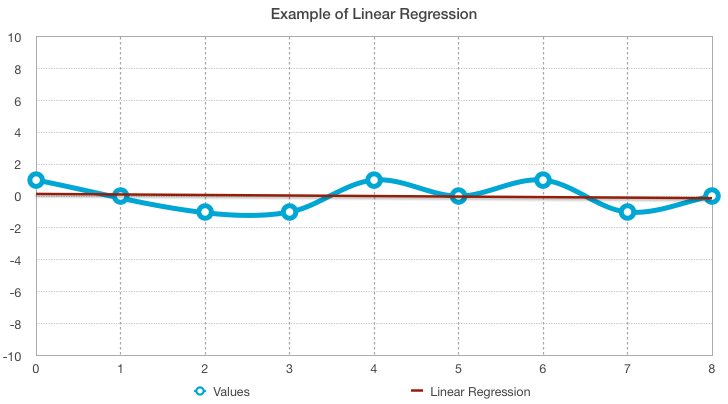
\includegraphics[width=100mm]{images/degree0.png}
%\caption{Example of Linear regression}
%\label{fig:degree0}
%\end{figure}

%Linear regression is polynomial regression of degree 1, and generally takes the form

%\begin{equation} \label{eq:polynomialFormSmall}
%f(x) = c_0 + c_1 * x
%\end{equation}

%where \emph{$c_0$} is the y-intercept and \emph{$c_1$} being the slope. Figure \ref{fig:degree1} shows clearly that the linear regression line running along the data points approximate the data. Mean average and linear regression are the most commom forms of polynomial regression, but not the only.

%\begin{figure}[ht!]
%\centering
%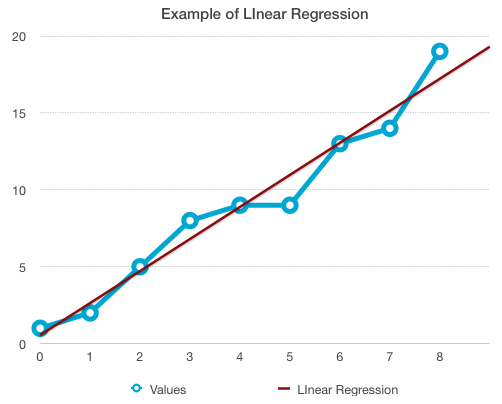
\includegraphics[width=100mm]{images/degree1.png}
%\caption{Example of Linear regression}
%\label{fig:degree1}
%\end{figure}

%The next step of polynomial would be the quadratic regression, now the regression becomes non-linear and the data is not restricted to straight lines. With figure \ref{fig:degree2} is possible to visualize a data with a quadratic regression trend line. Basically, the idea is simple: find a line that best fits the data which is find the coefficients to a polynomial that best fits the data.

%\begin{figure}[ht!]
%\centering
%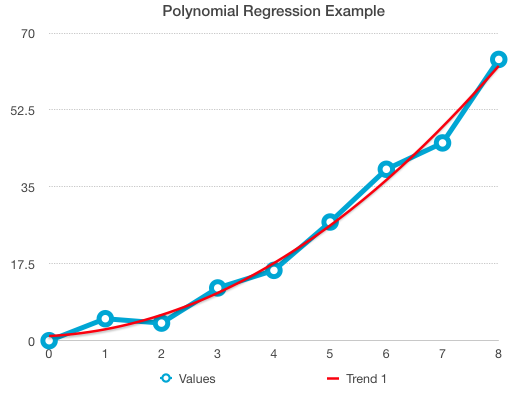
\includegraphics[width=100mm]{images/degree2.png}
%\caption{Example of Polynomial Regression}
%\label{fig:degree2}
%\end{figure}

%Polynomial regression is an overdetermined system of equations that uses least squares as a method of approximating an answer. To understand this, some linear algebra is required. 


%ACTIVITY OF A SOLUTE
\subsubsection{Activity of a solute}
Activity (\ce{a_i}) is \emph{"thermodynamic concentration"} (or informally known as \emph{"effective concentration"}). It is calculated as a product of activity coefficient and concentration (where \emph{i} means the solute involved):
\begin{equation}\label{activityEq}
a_i = \gamma_i * m_i
\end{equation}
Activity coefficient ($\gamma_i$) is a function of ionic strenght (I), which is a measure of the concentration of ions in the solution.  

%IONIC STRENGTH
\subsubsection{Ionic strength}
Mathematically the ionic strength of the solution is calculated according to
\begin{equation} \label{eq:ionicStrength}
I = 0.5 \sum{M_i z_i^2}
\end{equation}
where \emph{M} is the molar concentration of the specie \emph{i} having a charge \emph{z}.When \emph{I} increases, activity coefficients decrease. In very diluted solutions, activity coefficient is equals to \emph{1.0}, and activity is equal to concentration. The decreasing trend is related to the "cage" of opposite charge particles around ions. There is reversal of the trend in extremely concentrated solutions (brines), because beyond ionic strenght of about $1 mol/L$ there is an increase of activity coefficients with increasing ionic strength. This is related to decreasing amount of free water because most of water is already bound around dissolved species.
For a matter of explanation, we will calculate the ionic strength of a \ce{CaCl_2} solution (composed by $0.5 mol$ of \ce{Ca^{+2}} and $1 mol$ \ce{Cl^{-1}}):
\begin{eqnarray}
I = \frac{1}{2}  (z^2_{Ca}[Ca^{+2}]) + \frac{1}{2}  (z^2_{Cl}[Cl^{-1}]) \\
I = \frac{1}{2}  (2^2_{Ca}[Ca^{+2}] +  (-1)^2_{Cl}[Cl^{-1}]) \\
I = \frac{1}{2} (4 * 0.5 + 1 * 1) \\
I = 1.5 mol/L
\end{eqnarray}


%ACTIVITY COEFFICIENT
\subsubsection{Activity Coefficient} 
There are different methods to calculate $\gamma$ for ions:
\begin{itemize}
\item Debie-Hueckel: They assumed that ions behave like spheres with charges located at their center points. The ions interact with each other by coulombic forces and the result of their analysis is as follows
\begin{eqnarray} \label{eq:debyeEq}
log \gamma_i &=& - Az_i^2\sqrt{I}
\end{eqnarray} 
where \emph{A} is a constant that is a function of temperature, \emph{$z_i$} is the ion charge and \emph{I} is the ionic strength of the solution.
\item Davies equations: Is a variation of Debie-Hueckel that can be used when the ionic strength is relatively high. The equation is as follow
\begin{eqnarray} \label{eq:daviesEq}
log \gamma_i &=& - Az_i^2 \bigg(\frac{\sqrt{I}}{1+\sqrt{I}} - 0.3 I)
\end{eqnarray}
\item B-dot: This model is presented as an activity model based on an equation similar to Davies and parameterized for solutions up to 3 molal ionic strength.
\begin{eqnarray} \label{eq:bdotEq}
log \gamma_i &=& - \frac{Az_i^2 \sqrt{I}}{1+ a_i B \sqrt{I}} + \overset{.}{B} I )
\end{eqnarray}
where \emph{\aa}  is the ion size for each specie and \emph{A, B and $\overset{.}{B}$} are coefficients that vary with the temperature.
\end{itemize}
Important to mention that there are other methods available for calculating activity coefficients, which are not going to be addressed here. Pure solids have activity coefficient equal to one. Each one of the methods has its advantages and limitations. Debye-Hueckel equations are simple to apply, and is an extensible method for including new species in the solution due to the fact that it requires a low number of (specific) arguments. Moreover, Debye-Hueckel can be applied to the most important temperatures in the field of aqueous geochemistry, but it works poorly regarding moderate or high ionic strength.
As to dissolution and precipitation, there is clearly a reaction happening during these processes, which means that some reactions are not in equilibrium.

%SATURATION INDEX
\subsubsection{Saturation Index}
The saturation index (\emph{SI}) indicates the degree of saturation with respect to a given mineral; in other words, it defines if a reaction will be in equilibrium or not. \emph{SI} is expressed as
\begin{eqnarray} \label{eq:siEq}
SI &=& log (IAP / K )
\end{eqnarray}
When a mineral is in equilibrium within a solution, the \emph{SI} is zero: a negative \emph{SI} indicates undersaturation, and a positive \emph{SI}, supersaturation. 
The Ion Activity Product (\emph{IAP}) is calculated according to
\begin{eqnarray}
IAP &=& \frac{[C]^c [D]^d}{[A]^a[B]^b}
\end{eqnarray}
where [A], [B], [C] and [D] are activitys of each ion. The interpretation of \emph{IAP} is the following:
\begin{itemize}
\item IAP > K : The reaction is progressing from right to left, producing more products. In a ground water solution, the water is supersaturated.
\item IAP = K : The reaction is in equilibrium, there is no flow neither to the right nor to the left. In a ground water solution, the water and the mineral are in equilibrium.
\item IAP < K : The reaction is progressing from left to right, producing more reactants. In a ground water solution, the water is undersaturated.
\end{itemize}

With the \emph{SI} approach, it is possible to predict the reactive mineralogy of the subsurface from the ground-water data without collecting samples of the solid phase and analyzing the mineralogy. If the \emph{SI} for a mineral is less than zero, the aqueous solution is undersaturated with respect to that mineral - which corresponds to the fact that the mineral will not precipitate and may dissolve in order to reach equilibrium concentrations. If the \emph{SI} is greater than zero, then the mineral is not reactive and the mineral may precipitate from the aqueous solution (oversaturated). To conclude, when the \emph{SI} is close to zero (it is ok to consider a small range of values to be in equilibrium) , it means that the water is saturated  with respect to that mineral \cite{Alley:93}. From the mentioned before, it is possible to state the following:
\begin{itemize}
\item SI < 0 : Mineral is undersaturated;
\item SI = 0 : Mineral is in equilibrium with the solution;
\item SI > 0 : Mineral is oversaturated;
\end{itemize}

%HYDROGEOCHEMISTRY COMMON UNITS
\subsubsection{Hydrogeochemistry common units}
Molarity (\emph{M}) is defined as mass in moles in 1 liter of solution and molality (\emph{m}) is defined as mass in moles in 1 kilogram of solution. In dilute solutions, molarity is approximately equal to molality. Concentration in miliequivalents per liter is concentration in milimoles per liter multiplied by charge of an ion.

%HYDROCHEMICAL PROCESSES
\subsection{Hydrochemical processes}

%ACID-BASE REACTIONS
\subsubsection{Acid-Base Reactions}
The importance of acid-base reactions is cleary evident when one understands their influence on the pH. The pH is a master variable in charge of controlling chemical systems, and it is described as
\begin{eqnarray}
pH = - log([H^+])
\end{eqnarray}
where $[H^+]$ is the activity of the hydrogen ion. The interpretation of the values is as follows:
\begin{itemize}
\item pH < 7 : acid solution;
\item pH = 7 : neutral solution;
\item pH > 7 : basic solution;
\end{itemize}
The acid substance has a tendency to loose protons, while a basic substance has tendency to gain protons, and the interation between acids and bases is called acid-base reactions and is described as
\begin{eqnarray}
Acid_1 + Base_2 &=& Acid_2 + Base_1
\end{eqnarray}
The reaction must be understood as that in the forward reaction, the proton lost by $Acid_1$ is gained by $Base_2$ and, in the reverse reaction, the proton lost by $Acid_2$ is gained by $Base_1$.  The strength of an acid or base refers to the proportion of the protons that are lost or gained. 

%COMPLEXATION AND SPECIATION
\subsubsection{Complexation and Speciation}
Complexation is when an ion is formed by combining simpler cations, anions and sometimes molecules. This process facilitates the transport of potentially toxic substances and form what is called a complex. Due to the impact of this process in contamination problems, it has acquired a huge importance in practical and commercial fields. A simple example of complexation is the following
\begin{eqnarray}\label{complexation_reaction}
Mn^{2+} + Cl^- &=& MnCl^+
\end{eqnarray}
The calculation of the distribution of metals among complexes (\emph{speciation}) involves the solution of a series of mass-law transport equations. The mass-law equation of the reaction ~\ref{complexation_reaction} is described below
\begin{eqnarray}
K_{MnCl^+} &=& \frac{[MnCl^+]}{[Mn^{2+}][Cl^-]}
\end{eqnarray}
Each complex compound has a property called stability constant ($\beta_i$). It defines how the total concentration of the components are distributed among the possible compounds (it may include other complexes) in the solution.

%OXIDATION-REDUCTION REACTIONS
\subsubsection{Oxidation-Reduction Reactions}
Groundwater environment's reactions involve the transfer of electrons between its components (gaseous, dissolved or solid constituents). As a result, there are changes in the oxidation states of the reactants and products. It is important to stress that the oxidation number is a hypothetical charge that an atom would have if the ion or molecule were to dissociate. This state can be different according to the solution. 

In this work, \emph{redox reactions} (as oxidation-reduction reactions are also known) are not going to be addressed. In order to get deeper understanding on this topic, we refer to \cite{Petrucci:07}

%ADSORPTION AND ION EXCHANGE
\subsubsection{Adsorption and ion exchange}
Adsorption systems treat water by adding a substance, such as activated carbon or aluminia, to the water supply. Adsorbents attract contaminants by chemical and physical processes that cause them to \emph{stick} to their surfaces for later disposal. This mechanism is often used to remove contaminants like \emph{arsenic} or \emph{fluoride} (mostly organic contaminants) from water reservoirs. Ion exchange works simillarly but it is focused on inorganic contaminants in a particle-free water. Ion exchange is most often used to remove hardness or nitrate (mostly inorganic soluble molecules). 

In this work, adsorption and ion exchange are not going to be addressed. In order to get deeper understanding on this topic, we refer to \cite{Freeze:79}

% GEOCHEMICAL MODELLING
\subsection{Geochemical Modelling}
The geochemical modelling is the design of the geochemical reactions responsible for the migration of dissolved species. Geochemical models can be divided into two groups:
\begin{itemize}
\item Geochemical Equilibrium Models: Based on the assumption of thermodynamic equilibrium reached in a relatively short time (no time factor is included in calculation). It takes into consideration only equilibrium reactions.
\item Geochemical Kinetic Models: It takes into account also kinetic reactions and include the time factor. As kinetic data is measured experimentally, there still is a lack of kinetic data available for many geochemical processes. 
\end{itemize}

As mentioned before, this work will focus on the first one - \emph{geochemical equilibrium models}.

Inside geochemical equilibrium models we can mention three divisions: speciation models; inverse models (also called mass-balance models); forward models (also called reaction-path models); and reactive transport (coupled) models. Regarding the relation to spatial coordinates, geochemical equilibrium models are considered \emph{batch models} - which are basically closed vessels or reactors.

%GEOCHEMICAL SPECIATION MODELLING
\subsubsection{Geochemical Speciation Modelling}
Speciation represents modelling based in the equilibrium of a system. A geochemical speciation modelling program calculates the distribution of dissolved species between free ions and aqueous complexes and also saturation indexes for different minerals. Sodium, for example, can be present in water as a free ion \ce{Na^+}, and also in the form of complexes with anions:

\begin{equation}
\ce{Na^+}_{total} = \ce{NaCl}_{aq} + \ce{NaOH} + \ce{Na^+}
\end{equation}

where \ce{Na^+_{total}} is total sodium concentration from chemical analysis. \ce{Na^+_{total}} is a component (e.g., chemical formula unit used to describe a system) and \ce{Na^+}, \ce{NaCl_{aq}} and \ce{NaOH} are species (chemical entities which really exist in the system). 

Information about the distribution of dissolved species is important, for example, for risk assessment of contamination by metals, because toxicity of metals depends on their speciation in the solution. Carbonate complexes of metals, for example, are less toxic than their free ions.

Saturation index (SI) is used to determine the direction of geochemical processes. When \emph{SI > 0} the mineral precipitates from the water, and when \emph{SI < 0}, the mineral dissolves in contact with the water, if it is present in solid phase. Field data necessary for input of speciation program are temperature, pH and results from laboratory chemical analysis (results obtained from a sample of the solution of interest).

Common problems solved using speciation programs are: 
\begin{itemize}
\item There is a sample with high concentration of dissolved sodium and we need to know the distribution of sodium between \ce{Na^+} and different complexes (for example, \ce{{NaCl}_{aq}} or \ce{NaOH}) because different forms of sodium have different characteristics;
\item There are ground water samples that had been in contact with granitic masses and we want to verify the possibility of precipitation of minerals like \emph{Albite} (a plagioclase feldspar mineral whose formula is \emph{\ce{NaAlSi_{3}O_{8}}}).
\end{itemize}

Details of several available programs will be presented and discussed in chapter ~\ref{chapter:review}).

The development of our software \emph{SHPECK}, which is a geochemical speciation modelling software will be detailed, presented and thoroughly discussed in chapter~\ref{chapter:SHPECK}. 

%Also important to mention that this work is the first work that will completely guide anyone to generate a geochemical speciation modelling software from the ground.

%OTHER TYPES OF GEOCHEMICAL MODELLING
\subsubsection{Other Types Of Geochemical Modelling}
There are other types of geochemical equilibrium models, as mentioned before. For the sake of completeness, we summarize their characteristics below. 
\begin{itemize}
%INVERSE GEOCHEMICAL MODELLING
\item Inverse geochemical modelling
This type of models, also known as mass-balance models, are used when chemistry of groundwater and solid phase composition are already known, and reactions that have already happened should be determined. It is used when we have access to 2 hydraulically connected points and composition of solid phase between these points. With these data in hand, it is possible to calculate and produce the reactions that will explain the changes of the water's chemistry. This approach leads to some uncertainties: stoichiometry of minerals in solid phase is not often well known; solution may be non-unique; and programs can produce several possible models for the same input. An interesting work about inverse geochemical modelling is \cite{Sharif:07}.

%FORWARD GEOCHEMICAL MODELLING
\item Forward geochemical modelling
This type of models, also called reaction-path models, are used for prediction of water chemistry evolution along a flowline. The initial water chemistry is known and the aim of the program is to predict water chemistry at some point along the flow path. This kind of modelling introduces problems regarding kinetic and adsorption data, which are often missing and frequently limited.
\end{itemize}

\newpage

%SUMMARY
\section{Summary}
\begin{itemize}
\item Importance of multidisciplinary problems: The power from the advances in computer science to adapt itself to other areas of knowledge is ever increasing. The best way to push the limits of our work is by redefining obstacles outside our normal boundaries and reach solutions based on new understanding of complex situations. On the other hand, understanding what is a software and how it connects with the \emph{"machine world"} to the \emph{"real world"} is something non-trivial. We reinforce the idea that the extension of a software goes way beyond the lines of code and the interface showing up on the screen.We often find the comparison that building software is somehow like building a house - this certainly is a helpful example to understand everything that is behind a software. Both house and software require: estimating costs, thinking about the requirements, plans, rules, standards, best practices, specifications timelines, reviews, milestones, testing, alterations, handover and warranty.
\item Hydrogeochemistry principles: Thermodynamics is one of the substantial basis for the history of physics, chemistry and the science in general as we know it. It is crucial to understand the role that it has in the natural aspects of the world that we live. The comprehension of thermodynamics goes through the analysis, awareness and interrelations of the several factors that compose this complex \emph{maze}. From the wide range of factors, we can mention the equilibrium and kinetic reactions, the activity and the activity coefficient of the solute, the ionic strength of the solution, the saturation index, etc.
\end{itemize}